\documentclass{article}
\usepackage{graphicx} % \includegraphics
\usepackage{hyperref} % \href

\graphicspath{{./images/}}

\begin{document}
\title{
\includegraphics[scale=.2]{logo.png} \\[3ex] A.S.E - 2024/2025 \\ First Prototype Delivery}
\author{{\large \emph{EzGacha Team}} \\[1ex] Gioele Dimilta \\ Andrea Mugnai \\ Jacopo Tucci}
\date{}

\pagenumbering{gobble}
\maketitle

\newpage
\pagenumbering{arabic}
\tableofcontents

\newpage
\section{Introduction}
TBD...

\section{Architecture}
The architecture is based on microservices and each one implements a specific functionality. The overall structure is described in Figure \ref{fig:general_architecture}.
\begin{figure}[ht]
    \centering
    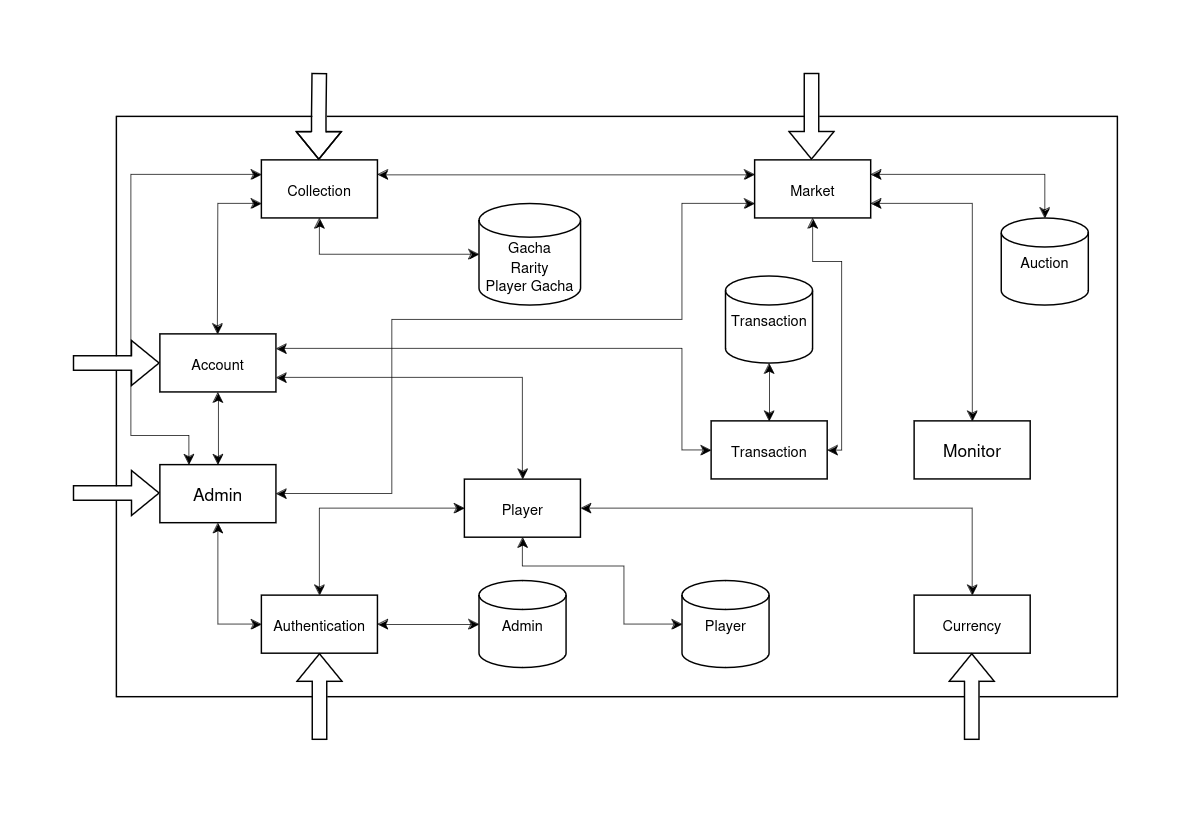
\includegraphics[width=12cm]{architecture-v2.drawio.png}
    \caption{General architecture}
    \label{fig:general_architecture}
\end{figure}

A player can register himself through the \emph{Account Service}. Then, he can login by \emph{Authentication Service}. After that, he can perform some operations inside the website, e.g.
\begin{itemize}
    \item Roll a gacha and check system gacha collection (\emph{Collection Service})
    \item Change password/username, retrieve his own gacha collection and check his transactions history (\emph{Account Service})
    \item Create an auction to sell a gacha and make bids on active auctions (\emph{Market Service})
    \item Purchase in-game currency (\emph{Currency Service})
\end{itemize}
Unlike the other services, \emph{Player Service} and \emph{Transaction Service} are not linked to the outside since they only manage the access to the databases (\emph{Player} and \emph{Transaction} tables). Players and admins can access only the API exposed by a \emph{CaddyServer} web reverse proxy, which allows to map specific services API to the outside. The login functionality is based on jwt tokens and each service can check the token validity to accept/discard an http request.

The \emph{RabbitMQ} message broker allows to send \emph{tasks} to the \emph{Celery Worker}. In order to manage the auction closing operation, \emph{Market Service} sends a new task to the worker, which will wait until auction expires before notify the service to close the auction.

\subsection{Architectural Smells}
The \emph{MicroFreshener} architecture is described in Figure \ref{fig:microfreshener_architecture}.
\begin{figure}[ht!]
    \centering
    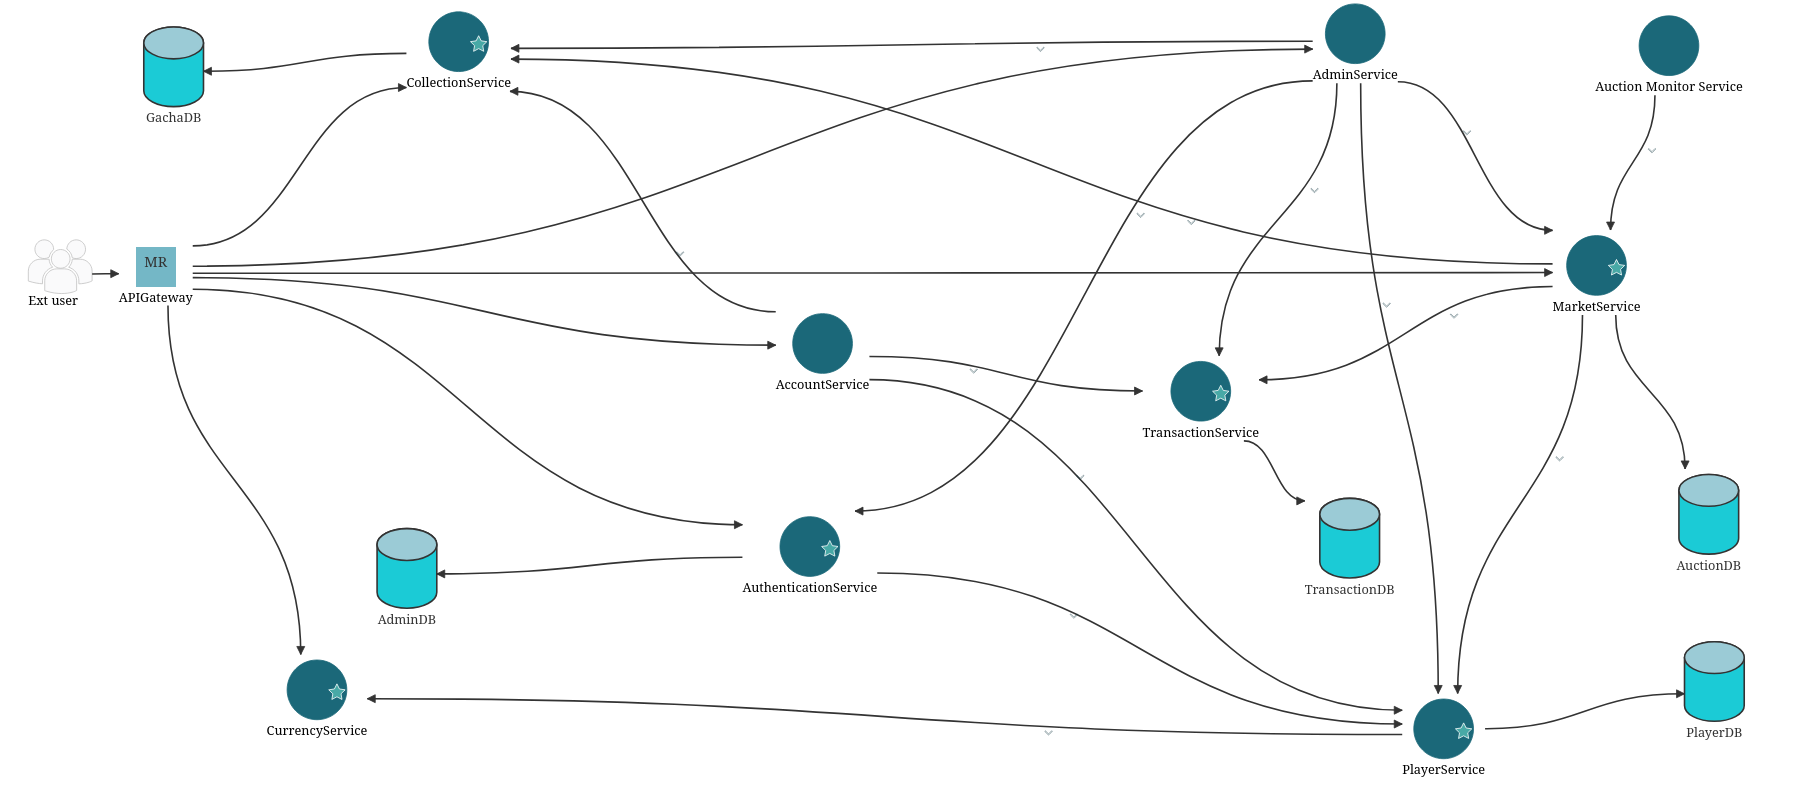
\includegraphics[width=12cm]{microFreshenerArchitecture.png}
    \caption{MicroFreshener architecture}
    \label{fig:microfreshener_architecture}
\end{figure}

Using the \emph{MicroFreshener} tool, we searched for architectural smells and we solved them accordingly. We used the \emph{circuit breaker} design pattern to handle the \emph{wobbly service interaction smell}. No additional smells came out during analysis phase.

\newpage
\subsection{Database}
Here is an E-R diagram of the previous monolithic database.
\begin{figure}[ht]
    \centering
    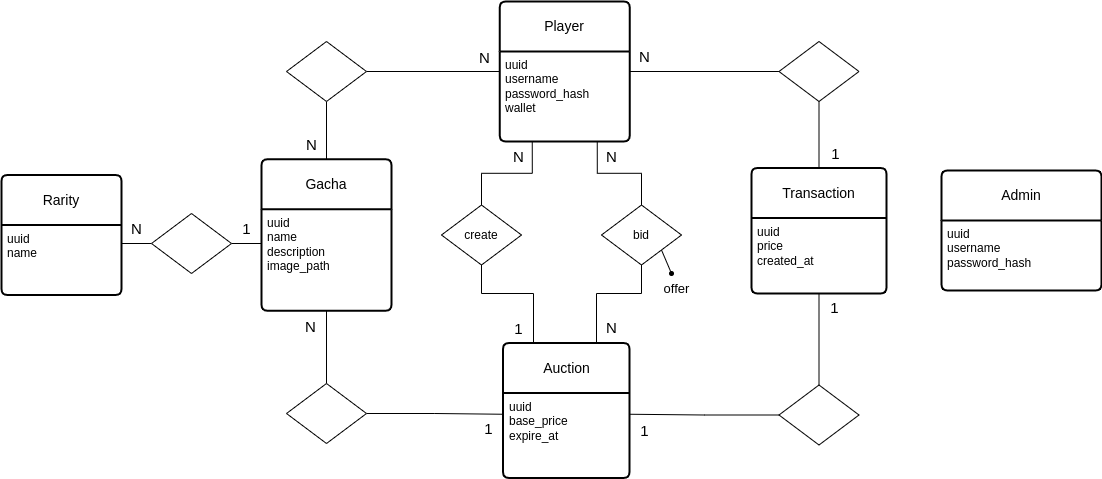
\includegraphics[width=12cm]{ASE-er-v5.drawio.png}
    \caption{Database structure}
\end{figure}

The \emph{N-to-N} relationship between \emph{Player} and \emph{Gacha} will be implemented with the table \emph{Player\_Gacha}. The \emph{Bid} table expresses the \emph{N-to-N} relationship between \emph{Player} and \emph{Auction}. Since the architecture is now based on microservices, the database has been splitted as follow.
\begin{table}[ht!]
    \centering
    \begin{tabular}{|c|c|}
        \hline
        \textbf{Service} & \textbf{Database tables}     \\
        \hline
        Player           & Player                       \\
        Authentication   & Admin                        \\
        Collection       & Gacha, Rarity, Gacha\_Player \\
        Transaction      & Transaction                  \\
        Market           & Auction, Bid                 \\
        \hline
    \end{tabular}
    %\caption{Splitted database}
\end{table}

%\begin{itemize}
%    \item \emph{Gacha}, \emph{Rarity} and \emph{Gacha\_Player} tables are now controlled by \emph{Gacha Service}.
%    \item \emph{Player} table is now controlled by \emph{Player Service}.
%    \item \emph{Transaction} table is now controlled by \emph{Transaction Service}.
%    \item \emph{Auction} and \emph{Bid} tables are now controlled by \emph{Market Service}.
%    \item \emph{Admin} table is now controlled by \emph{Authentication Service}.
%\end{itemize}

\subsection{Services}
\textbf{Player Service} and \textbf{Transaction Service} act as database managers for \emph{Player} and \emph{Transaction} tables respectively. In particular, they provide basic CRUD APIs to interact with those tables, i.e. GET, POST, PUT and DELETE methods to fetch, insert, modify and delete records.

The \textbf{Authentication Service} allows players and admins to login and logout. It creates a jwt token if credentials are correct. Moreover, the admin token contains a boolean attribute \emph{is\_admin}. Admin authentication is done by \textbf{Admin service}. In particular, when an admin wants to login, he communicates with Admin Service, which sends a request to the Authentication Service. In this way, we can keep admin functionalities separated from the player.

The \textbf{Account Service} allows players to manage their account, see their gacha collection (actually passing by \emph{Gacha Service}) and transaction history. In particular, a player can modify and delete his account.

The \textbf{Currency Service} allows player to purchase in-game currency. A player can specify the amount of currency he wants to get and his wallet will be updated accordingly.

The \textbf{Collection Service} manages the system gacha collection and the related rarities. Also, it controls the \emph{Player\_gacha} table, which contains the infos about all the player collections. Therefore, the account service must communicate with collection service when the user wants to retrieve his collection. The collection service provides also the \emph{roll} functionality, which returns a gacha according to the following probabilities.

\begin{table}[ht!]
    \centering
    \begin{tabular}{|c|c|c|c|c|}
        \hline
        \textbf{Common} & \textbf{Uncommon} & \textbf{Rare} & \textbf{Epic} & \textbf{Legendary} \\
        \hline
        $50\%$          & $30\%$            & $10\%$        & $8\%$         & $2\%$              \\
        \hline
    \end{tabular}
    %\caption{Rarity probabilities}
\end{table}

%\begin{itemize}
%    \item Common (C): $50\%$
%    \item Uncommon (UC): $30\%$
%    \item Rare (R): $10\%$
%    \item Epic (E): $8\%$
%    \item Legendary (S): $2\%$
%\end{itemize}

The \textbf{Market Service} is the most complex component of the architecture. It manages auctions, bids and payments. When a player creates a new auction, the service sends a task to the \emph{Celery Worker} in order to guarantee that the auction ends when expire time comes. In particular, the worker will do a POST request to \emph{/payment} market API and the service will close the auction managing both the payment operations and gacha transfer from seller to buyer. If the payment is successfull, a new transaction record is created.

\section{Use Cases}
\subsection{User login}
The player wants to login into the application.
\begin{enumerate}
    \item The player sends a POST request to the reverse proxy at \emph{/login} with username and password.
    \item The proxy forwards the request to the \emph{Authentication Service}.
    \item The microservice checks if the user is already logged. If not, it sends a GET request to the \emph{Player Service} at \emph{/username/<username>} to retrieve the player informations.
    \item The \emph{Player Service} retrieves user data from the database and sends them to the \emph{Authentication Service}.
    \item It checks if the password is not wrong and, if so, it generates a JWT session token.
    \item An http response containing the session token will be sent back to the proxy, which will forward it to the user.
\end{enumerate}

\subsection{User create auction}
The player wants to create a new auction.
\begin{enumerate}
    \item The player sends a POST request to the reverse proxy at \emph{/market} with the required data: the UUID of the gacha to be auctioned and the starting price.
    \item The proxy forwards the request to the \emph{Market Service}.
    \item The microservice checks the presence and validity of the JWT session token from the request cookie and extracts the player's UUID from the token payload.
    \item The \emph{Market Service} sends a GET request to the \emph{Player Service} at \emph{/uuid/<player\_uuid>}. 
    \item The \emph{Player Service} retrieves the player's ID and send back to the \emph{Market Service}.
    \item The microservice retrieves the player's gacha collection by sending a GET request to the \emph{Gacha Service} at \emph{/collection/user/<player\_id>}.
    \item Then \emph{Market Service} verifies if the player owns the specified \emph{gacha\_uuid} in sufficient quantity and checks the database for active auctions of the same item.
    \item If the player does not own the item or the number of active auctions matches or exceeds the available quantity, an error is returned.
    \item If all checks pass, a new auction is inserted into the database with a unique UUID, the specified starting price, and the auction's expiration time.
    \item After inserting the auction, the microservice retrieves the details of the created auction from the database, and a background task is scheduled using \emph{invoke\_payment} to handle auction's expiration.
    \item An HTTP response containing the created auction's details is sent back to the proxy, which forwards it to the user.
\end{enumerate}

\section{How to run}
The application has been virtualized using \emph{Docker}. Each component (services, databases, message brokers, etc.) is a container and we can manage them with \emph{Docker Compose}. In order to run the application, clone the github repo and enter inside \emph{src/} directory. Then, build the images and run the containers.
\begin{verbatim}
    git clone https://github.com/pklone/ASE-project.git
    cd ASE-project/src
    docker compose up -d --build
\end{verbatim}
The application is accessible from the proxy end-point at
\begin{verbatim}
    https://ase.localhost
\end{verbatim}
At the moment, no web GUI is available. However, you can use tools like \emph{curl} to interact with the application. Check the \href{https://github.com/pklone/ASE-project/test/README.md}{github repo} for examples.
\end{document}
